\documentclass[apj]{aastex62}
\shorttitle{Delay Time Distributions of SNe~Ia}
\shortauthors{Strolger et al.}

\usepackage{natbib}
\usepackage{nicefrac}
\usepackage{ulem}
\usepackage{xcolor}
\usepackage{topcapt}
\usepackage{amssymb,amsmath}
\bibliographystyle{apj}

\renewcommand{\deg}{^{\circ}}
\begin{document}
\title{The Empirical Delay Time Distributions of Type Ia Supernovae From Galaxy and Cosmic Star Formation Histories}
\author[0000-0002-7756-4440]{L.-G.~Strolger}
\author{Steven Rodney}
\author{Camila Pacifici}
\author{et al.}

\begin{abstract}
blah, blah, blah \ldots
\end{abstract}

\section{Introduction}
Understanding cosmic type Ia supernova (SN~Ia) rates have a critical importance to understanding galaxy evolutionary feedback mechanisms, the cosmic iron enrichment and $\alpha$-process element enrichment histories \citep{Maoz:2017ck}, and constraining the physical mechanisms of SN~Ia progenitors. However, tracing rate histories has been a slog, with the first precise measures of the local ($z\approx0.0$) rate in the early 1990s \cite[cf.][]{Cappellaro:1993qm,Cappellaro:1997,Cappellaro:1999}, and the first measures beyond the Hubble flow beginning in the early 2000s as a result of the dark energy experiment~\citep{Riess:1998,Perlmutter:1999}. Since then, there have been several measures of the volumetric SN~Ia rate at various redshifts by various groups. These rate values have not always been in total agreement with one another, and there may be several valid reasons as to why (see rev. by Haden?). For the time being it probably best to consider each published rate value as a valid measure. Further, we assume each is valid within their measured statistical error, which again may be bold, but is probably satisfactory given the number of rate measures in each redshift interval. A collection of volumetric SN~Ia rates is shown in Figure~\ref{fig:sn1a_rates} and in Table~\ref{tab:sn1a_rates}. 
\begin{figure}[t]
   \centering
   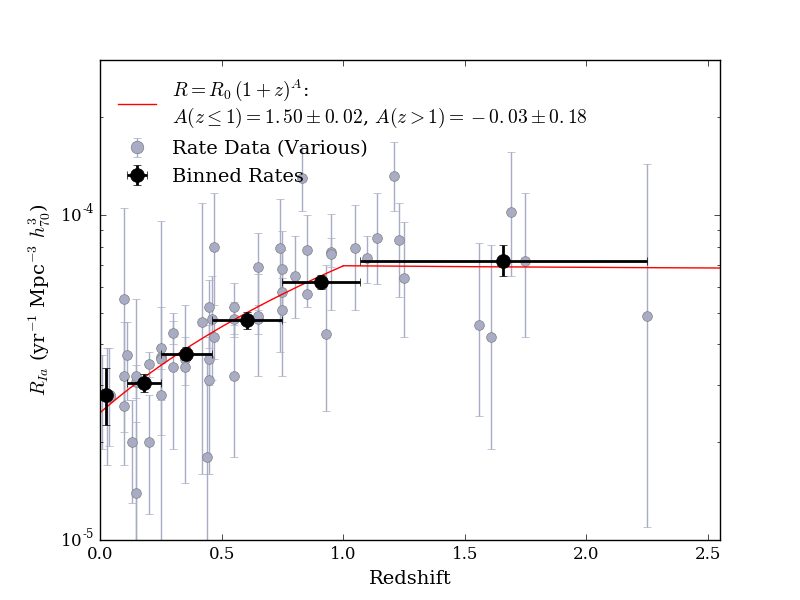
\includegraphics[width=6.1in]{figure_SNIa_rate_z_pwr_fit}
   \caption{\footnotesize Type Ia supernova volumetric rate measures from various sources in the literature (gray points, see Table~\ref{tab:sn1a_rates} for their sources), and binned (black points, see Table~\ref{tab:sn1a_bin}), largely for illustration. Red lines show a broken power-law fit to the data in redshift space.}
   \label{fig:sn1a_rates}
\end{figure}


\startlongtable
\begin{deluxetable}{lcccl}
\tablecaption{Volumetric SN Ia Rates Used in this Work}
\tablehead{
\colhead{Redshift} & \colhead{$R_{\rm Ia}$\tablenotemark{a}} &\colhead{Stat. Uncertainty} & \colhead{Sys. Uncertainty} & \colhead{Source}}

%	 &$R_{Ia}$ & Statistical & Systematic &\\
%	Redshift & $(10^{-4}$ yr$^{-1}$ Mpc$^{-3}$ $h_{70}^3)$ & Uncertainty & Uncertainty& Source \\

\startdata
0.01&0.28&$^{+0.09}_{-0.09}$&$^{+0.0}_{-0.0}$&\cite{Cappellaro:1999}\\
0.03&0.28&$^{+0.11}_{-0.11}$&$^{+0.0}_{-0.0}$&\cite{Mannucci:2005}\\
0.0375&0.278&$^{+0.112}_{-0.083}$&$^{+0.015}_{-0.00}$&\cite{Dilday:2010}\\
0.1&0.259&$^{+0.052}_{-0.044}$&$^{+0.028}_{-0.001}$&\cite{Dilday:2010}\\
0.10&0.32&$^{+0.15}_{-0.15}$&$^{+0.0}_{-0.0}$&\cite{Madgwick:2003}\\
0.10&0.55&$^{+0.50}_{-0.29}$&$^{+0.20}_{-0.20}$&\cite{Cappellaro:2015oq}\\
0.11&0.37&$^{+0.10}_{-0.10}$&$^{+0.0}_{-0.0}$&\cite{strolger2003}\\
0.13&0.20&$^{+0.07}_{-0.07}$&$^{+0.05}_{-0.05}$&\cite{Blanc:2004}\\
0.15&0.307&$^{+0.038}_{-0.034}$&$^{+0.035}_{-0.005}$&\cite{Dilday:2010}\\
0.15&0.32&$^{+0.23}_{-0.23}$&$^{+0.23}_{-0.06}$&\cite{Rodney:2010b}\\
0.16&0.14&$^{+0.09}_{-0.09}$&$^{+0.06}_{-0.12}$&\cite{Perrett:2012}\\
0.2&0.348&$^{+0.032}_{-0.030}$&$^{+0.082}_{-0.007}$&\cite{Dilday:2010}\\
0.20&0.20&$^{+0.08}_{-0.08}$&$^{+0.0}_{-0.0}$&\cite{Horesh:2008}\\
0.25&0.36&$^{+0.60}_{-0.26}$&$^{+0.12}_{-0.35}$&\cite{Rodney:2014fj}\\
0.25&0.365&$^{+0.031}_{-0.028}$&$^{+0.182}_{-0.012}$&\cite{Dilday:2010}\\
0.25&0.39&$^{+0.13}_{-0.12}$&$^{+0.10}_{-0.10}$&\cite{Cappellaro:2015oq}\\
0.26&0.28&$^{+0.07}_{-0.07}$&$^{+0.06}_{-0.07}$&\cite{Perrett:2012}\\
0.30&0.34&$^{+0.16}_{-0.15}$&$^{+0.0}_{-0.0}$&\cite{Botticella:2008}\\
0.30&0.434&$^{+0.037}_{-0.034}$&$^{+0.396}_{-0.016}$&\cite{Dilday:2010}\\
0.35&0.34&$^{+0.19}_{-0.19}$&$^{+0.19}_{-0.03}$&\cite{Rodney:2010b}\\
0.35&0.36&$^{+0.06}_{-0.06}$&$^{+0.05}_{-0.06}$&\cite{Perrett:2012}\\
0.42&0.46&$^{+0.42}_{-0.32}$&$^{+ 0.10}_{-0.13}$&\cite{Graur:2014}\\
0.44&0.262&$^{+ 0.229}_{-0.133}$&$^{+ 0.059}_{-0.120}$&\cite{Okumura:2014}\\
0.45&0.31&$^{+0.15}_{-0.15}$&$^{+0.15}_{-0.04}$&\cite{Rodney:2010b}\\
0.45&0.36&$^{+0.06}_{-0.06}$&$^{+0.04}_{-0.05}$&\cite{Perrett:2012}\\
0.45&0.52&$^{+0.11}_{-0.13}$&$^{+0.16}_{-0.16}$&\cite{Cappellaro:2015oq}\\
0.46&0.48&$^{+0.17}_{-0.17}$&$^{+0.0}_{-0.0}$&\cite{Tonry:2003}\\
0.47&0.42&$^{+0.06}_{-0.06}$&$^{+0.13}_{-0.09}$&\cite{Neill:2006}\\
0.47&0.80&$^{+0.37}_{-0.27}$&$^{+1.66}_{-0.26}$&\cite{Dahlen:2008}\\
0.55&0.32&$^{+0.14}_{-0.14}$&$^{+0.14}_{-0.07}$&\cite{Rodney:2010b}\\
0.55&0.48&$^{+0.06}_{-0.06}$&$^{+0.04}_{-0.05}$&\cite{Perrett:2012}\\
0.55&0.52&$^{+0.10}_{-0.09}$&$^{+0.0}_{-0.0}$&\cite{Pain:2002}\\
0.65&0.48&$^{+0.05}_{-0.05}$&$^{+0.04}_{-0.06}$&\cite{Perrett:2012}\\
0.65&0.49&$^{+0.17}_{-0.17}$&$^{+0.17}_{-0.08}$&\cite{Rodney:2010b}\\
0.65&0.69&$^{+0.19}_{-0.18}$&$^{+0.27}_{-0.27}$&\cite{Cappellaro:2015oq}\\
0.74&0.79&$^{+0.33}_{-0.41}$&$^{+0.0}_{-0.0}$&\cite{Graur:2011}\\
0.75&0.51&$^{+0.27}_{-0.19}$&$^{+0.23}_{-0.19}$&\cite{Rodney:2014fj}\\
0.75&0.58&$^{+0.06}_{-0.06}$&$^{+0.05}_{-0.07}$&\cite{Perrett:2012}\\
0.75&0.68&$^{+0.21}_{-0.21}$&$^{+0.21}_{-0.14}$&\cite{Rodney:2010b}\\
0.80&0.839&$^{+ 0.230}_{-0.185}$&$^{+ 0.060}_{-0.120}$&\cite{Okumura:2014}\\
0.83&1.30&$^{+0.33}_{-0.27}$&$^{+0.73}_{-0.51}$&\cite{Dahlen:2008}\\
0.85&0.57&$^{+0.05}_{-0.05}$&$^{+0.06}_{-0.07}$&\cite{Perrett:2012}\\
0.85&0.78&$^{+0.22}_{-0.22}$&$^{+0.22}_{-0.16}$&\cite{Rodney:2010b}\\
0.94&0.45&$^{+0.22}_{-0.19}$&$^{+ 0.13}_{-0.06}$&\cite{Graur:2014}\\
0.95&0.76&$^{+0.25}_{-0.25}$&$^{+0.25}_{-0.26}$&\cite{Rodney:2010b}\\
0.95&0.77&$^{+0.08}_{-0.08}$&$^{+0.10}_{-0.12}$&\cite{Perrett:2012}\\
1.05&0.79&$^{+0.28}_{-0.28}$&$^{+0.28}_{-0.41}$&\cite{Rodney:2010b}\\
1.1&0.74&$^{+0.12}_{-0.12}$&$^{+0.10}_{-0.13}$&\cite{Perrett:2012}\\
1.14&0.705&$^{+ 0.239}_{-0.183}$&$^{+ 0.102}_{-0.103}$&\cite{Okumura:2014}\\
1.21&1.32&$^{+0.36}_{-0.29}$&$^{+0.38}_{-0.32}$&\cite{Dahlen:2008}\\
1.23&0.84&$^{+0.25}_{-0.28}$&$^{+0.0}_{-0.0}$&\cite{Graur:2011}\\
1.25&0.64&$^{+0.31}_{-0.22}$&$^{+0.34}_{-0.23}$&\cite{Rodney:2014fj}\\
1.59&0.45&$^{+0.34}_{-0.22}$&$^{+ 0.05}_{-0.09}$&\cite{Graur:2014}\\
1.61&0.42&$^{+0.39}_{-0.23}$&$^{+0.19}_{-0.14}$&\cite{Dahlen:2008}\\
1.69&1.02&$^{+0.54}_{-0.37}$&$^{+0.0}_{-0.0}$&\cite{Graur:2011}\\
1.75&0.72&$^{+0.45}_{-0.30}$&$^{+0.50}_{-0.28}$&\cite{Rodney:2014fj}\\
2.25&0.49&$^{+0.95}_{-0.38}$&$^{+0.45}_{-0.24}$&\cite{Rodney:2014fj}\\
\enddata
\tablenotetext{a}{In units $10^{-4}$ yr$^{-1}$ Mpc$^{-3}$ $h_{70}^3$}
\label{tab:sn1a_rates}
\end{deluxetable}


\begin{table}[h]
   \centering
   \caption{Binned volumetric SN~Ia rates, with statistical uncertainties.}
   \begin{tabular}{lc} 
   \hline
   \hline
   Redshift & $R_{\rm Ia}$\tablenotemark{a}\\
   \hline
$0.07 \pm{0.06}$ & $0.28^{+0.04}_{-0.03}$\\
$0.19 \pm{0.06}$ & $0.30^{+0.02}_{-0.02}$\\
$0.33 \pm{0.08}$ & $0.38^{+0.02}_{-0.02}$\\
$0.44 \pm{0.03}$ & $0.35^{+0.05}_{-0.04}$\\
$0.61 \pm{0.14}$ & $0.47^{+0.03}_{-0.03}$\\
$0.81 \pm{0.07}$ & $0.60^{+0.04}_{-0.04}$\\
$1.05 \pm{0.17}$ & $0.76^{+0.06}_{-0.06}$\\
$1.73 \pm{0.52}$ & $0.61^{+0.14}_{-0.10}$\\
\hline
   \end{tabular}
   \tablenotetext{a}{In units $10^{-4}$ yr$^{-1}$ Mpc$^{-3}$ $h_{70}^3$}
   \label{tab:sn1a_bin}
\end{table}

It would be reasonable to assume the volumetric rates follow a broken power law evolution with redshift, i.e., $R_{Ia}=R_0\,(1+z)^A$ where at $z<1$ the power-law slope is $A=1.50\pm0.02$ (with $R_0 = 2.47\pm0.02\times10^{-5}$ yr$^{-1}$ Mpc$^{-3}$ $h_{70}^3$), which flattens substantially to $A=-0.06\pm0.2$ at redshifts greater than 1, as is shown in  Figure~\ref{fig:sn1a_rates}. This is broadly consistent with the power-law fit of \cite{Okumura:2014}, and the locus with the measured SN~Ia rate at $z\approx0$ from \cite{Li:2011b} of approximately $2.7\pm0.3\times10^{-5}$ yr$^{-1}$. 


\section{Delay Time Distributions from Volumetric SN~Ia Rates and the Cosmic Star Formation History}

For these types of analyses, the standard assumption is that the stellar death rate (or supernova rate) is related to the stellar birth rate, convolved with some delay-time distribution that contains all the temporal factors of stellar evolution (e.g., main sequence lifetime, etc.) and binary star evolution (e.g., accretion rates or merger times). Two additional terms include the fraction of the initial mass function (or IMF) that are the progenitors to the SNe~Ia (presumably $3 - 8\, \rm{M}_{\odot}$ zero-age main sequence stars, see discussion in Section~\ref{sec:wds}), and the fraction of that population that are actually capable of producing events, as not are necessarily in the right type of binary system or systems.

We can relate volumetric SN~Ia rate history to the cosmic star formation history($\dot{\rho}_{\star}$) in a similar way, expressed mathematically by, 
\begin{equation}
R_{\rm Ia}(t) =  h^2\,k\,\varepsilon\,\biggl[\dot{\rho}_{\star}(t) \ast \Phi(t)\biggr],
\label{eqn:std}
\end{equation}
\noindent where $\Phi(t)$ is the delay-time distribution of SNe~Ia, $k$ is the fraction of the IMF (by mass) responsible for SN~Ia progenitors, $\varepsilon$ is the fraction of that population that are ultimately successful in producing SNe~Ia, and $t$ is the forward-moving clock of the universe. 

\subsection{The Fraction of Stars Responsible for SNe~Ia}~\label{sec:wds}
Dissecting each of these terms, $k$ is perhaps the easiest to approximate. The progenitors of SNe~Ia have traditionally been CO WD which acquire sufficient mass to approach or exceed the Chandrasekhar mass limit, $M_{ch}=1.44\,M_{\odot}$. To only marginally achieve this, they can either start at sufficiently high mass to require only a small amount of accretion from a nearby companion (typically single-degenerate, or SD, scenarios), or as a pair of WD that have combined in mass to meet this criterion (the double-degenerate, or DD, scenario) setting an even lower constraint~\cite[see][ for a review]{Maoz:2013}. In the case of WD/WD mergers, WD mass distributions are strongly peaked around $M_{\rm WD}\approx0.6\pm0.1\,M_{\odot}$ \citep{Catalan:2008il}, in which a pair drawn from such distribution may be satisfactorily close to the ignition threshold of a carbon core for a non-rotating CO WD, approximately $1.38\, M_{\odot}$ \citep{Arnett:1969dw, Nomoto:1982vh}. Initial-Final Mass relations \cite[e.g.,][]{Catalan:2008il,Cummings:2018oe} would correspond these to ZAMS masses of approximately $3\, M_{\odot}$, but no less than $\sim2.5\, M_{\odot}$. 

The same Initial-Final Mass relations would suggest that a WD essentially at $M_{ch}$ would fall just below $8\, M_{\odot}$ ZAMS. On a more physical bases, simulations show that the lowest mass in which C ignition is still possible is around $6-8 \,M_{\odot}$~\cite{Chen:2014rb,Denissenkov:2015rf}, but likely no more than $\sim11\, M_{\odot}$ \citep{Takahashi:2013jx}, above which an electron-capture-induced collapse mechanism begins, marking the onset of core-collapse supernovae.

It is reasonable, therefore, to assume a progenitor mass range of about $3-8\,M_{\odot}$ ZAMS. From a numerical assessment of these stars, assuming they fall within an IMF that is a power-law distribution by mass (in this initial mass range) with $\alpha\approx-2.3$~\citep{Salpeter:1955rw,Kroupa:2001gf}, one would expect 
\begin{equation}
k = \frac{\int\limits_{3M_{\odot}}^{8M_{\odot}} \xi(M)\,dM}{\int\limits_{0.1M_{\odot}}^{125M_{\odot}} M\,\xi(M)\,dM},
\end{equation}
\noindent where $k = 0.021^{+33\%}_{-24\%}\,M_{\odot}^{-1}$. The error in $k$ is driven more by choices in the upper and lower value in the selected mass range of  SN~Ia progenitors than by the choice in IMF model, as described above.

The fraction of CO WDs that are successful in making SNe~Ia is hard to determine, as we don't quite yet know the details of the progenitor mechanism or mechanisms. Estimates swing rather wildly from (perhaps) from as low as 1 in 200~\citep{Breedt:2017rp} to as optimistic as 1 in 40~\citep{Maoz:2012}. There is at least strong consensus that accretion on to a CO WD is essential, but very different plausible WD close binary scenarios from at least a theoretical standpoint~\citep{Nelemans:2001hb,Nelemans:2001cs}. The binary fractions of WDs has been recently estimated from the  the ESO-VLT Supernova-Ia Progenitor Survey~\citep[ SPY]{Napiwotzki:2007} show close double WD systems may have $\varepsilon_{\rm bin}\simeq0.1\pm0.02$, with separations distributed following a power-law slope of $\alpha=-1.3\pm15\%$~\citep{Maoz:2017zl}. It is not likely all of these successfully yield SNe~Ia as their merger rates in the MW are at least a magnitude higher than best estimates of the SN~Ia rate in our galaxy, and presumably some of these will form AM CVn and R~Corona Borealis stars, but at least it could be treated as an upper limit on $\varepsilon$.

\subsection{The star-formation density history}
The cosmic star formation history (CSFH), at least to $z < 5$, or over 90\% of the history of the universe, is fairly well understood, with~\cite[][ MD14 hereafter]{Madau:2014fk} providing one of the most complete compilations. More recently, the CSFH derived from the combined GAMA, G10-COSMOS, and 3D-HST datasets by~\cite{Driver:2018nr}, in a quasi-homogeneous analysis over a larger area, provides a dataset with greatly reduced uncertainties per datum, but fewer data than cited in the MD14 compendium (see Figure~\ref{fig:csfhs}).  We combine the MD14 and \cite{Driver:2018nr} data, with additional star-formation rate densities from \cite{Bouwens:2015qy} and \cite{Khusanova:2019kx}, to arrive at today's compendium CSFH using the parameterization,
\begin{equation}
\dot{\rho}_{\star}(z) = \frac{A\,(1+z)^C}{((1+z)/B)^D+1}.\label{eqn:mdp}
\end{equation}

\begin{figure}[t]
   \centering
   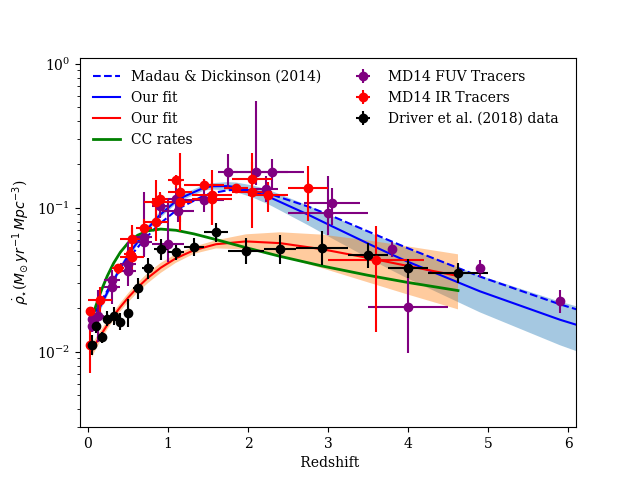
\includegraphics[width=6.1in]{figure_csfh_today}
   \caption{\footnotesize Shown are a compendium of cosmic star formation histories, from ~\cite{Madau:2014fk}, \cite{Driver:2018nr}, \cite{Bouwens:2015qy}, and \cite{Khusanova:2019kx}. Dashed lines (and associated shaded regions) are previous models  from \cite{Madau:2014fk}, \cite{Finkelstein:2014fj}, \cite{Strolger:2015aa}, as indicated. Solid blue line (and blue shaded region) represent our best-fit model to the compendium of data.}
   \label{fig:csfhs}
\end{figure}

We first correct the \cite{Driver:2018nr} data for dust attenuation following the prescription in MD14, by applying 
\begin{equation}
	\dot{\rho}_{\star}(z) =h^3\,\biggl[1+10^{0.4\cdot A_{\rm FUV}(z)}\biggr]\, \dot{\rho}_{\star, {\rm uncorrected}}(z),
\end{equation}
where it is assumed $A_{\rm FUV}(z)$ has essentially the same functional form of Equation~\ref{eqn:mdp}, and when applied to the MD14 $A_{\rm FUV}(z)$ data results in a Levenberg-Marquardt least-squares solution of $A=1.4\pm0.1$, $B=3.5\pm0.4$, $C=0.7\pm0.2$, and $D=4.3\pm0.7$. We then fit Equation~\ref{eqn:mdp} to the combined CSFH datasets,    resulting in parameters which are shown in Table~\ref{tab:csfh_fits} and Figure~\ref{fig:csfhs}. 

\begin{table}[h]
    \centering
    \caption{Cosmic Star Formation History Parameter Fits}
    \label{tab:csfh_fits}
    \begin{tabular}{lcccc}
         & $A$ & $B$ & $C$ & $D$ \\
        \hline
        \hline
	\cite{Madau:2014fk} only & $0.013 \pm 0.001$ & $2.6 \pm 0.1$ & $3.2 \pm 0.2$ & $6.1 \pm 0.2$\\
	\cite{Driver:2018nr} only & $0.014 \pm 0.001$ & $2.5 \pm 0.2$ & $3.3 \pm 0.3$ & $6.2 \pm 0.3$\\
	\hline
	All Combined Data & $0.0134 \pm 0.0009$ & $2.55 \pm 0.09$ & $3.3 \pm 0.2$ & $6.1 \pm 0.2$\\
	\hline
    \end{tabular}
\end{table}

\subsection{SN~Ia Progenitor Delay-Time Distribution Models}
\noindent [NOTE: talk about the expected delay-time distribution, values from Graur and Maoz, inability to probe turnover at `SN high noon', around $z\sim1$.]

\begin{figure}[t]
   \centering
   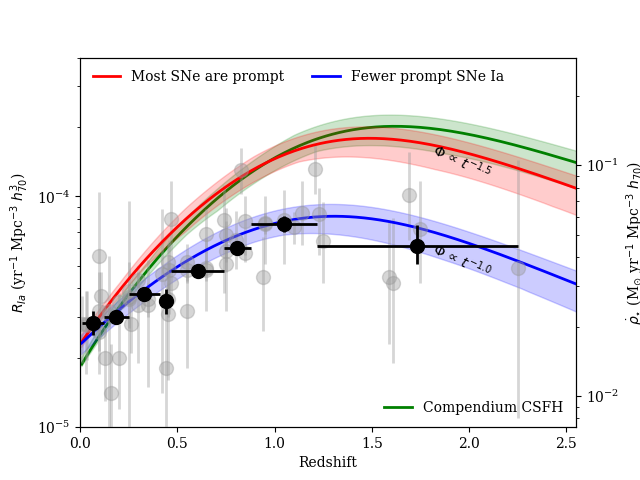
\includegraphics[width=6.1in]{figure_SNIa_rate_alpha}
   \caption{\footnotesize Shown in comparison to the data are the expected volumetric rates for power-law delay-time distributions ($\alpha = 1.0$ and 1.5 in red and blue, respectively) as applied to the cosmic star formation rates~\cite[in  solid and dashed green, respectively]{Madau:2014fk,Driver:2018nr}. Dashed rate models require a higher fraction of WD progenitors than the solid lines.}
   \label{fig:sn1a_rates2}
\end{figure}

Following \cite{Strolger:2010}, we can continue to test a robust delay-time model, capable of reproducing the theoretical distributions for SD and DD models at one extreme, and $\delta$-function delay times at the other. The unimodal, skew-normal $\Phi(\tau)$ function is defined as:

\begin{equation}
	\Phi(\tau)=\frac{1}{\omega\pi}\,\exp\biggl(\frac{-(\tau-\xi)^2}{2\omega^2}\biggr)\int_{-\infty}^{\alpha (\frac{\tau-\xi}{\omega})} \exp\biggl(\frac{-t'^2}{2}\biggr)\,dt',
\label{eqn:model}
\end{equation}

\noindent where location ($\xi$),\footnote{Different from the initial mass function, $\xi(M)$.} width ($\omega^2$), and shape ($\alpha$) are defined by the model. Figure~\ref{fig:dtd_families} demonstrates the flexibility of the model in producing various distributions in $\tau$.

%define the mode time ($\bar{\tau}$), variance ($\sigma^2$), skewness ($\gamma_1$), and kurtosis ($\gamma_2$) of the model function by,
%
%\begin{eqnarray*}
%\bar{\tau}&=&\xi+\omega\delta\sqrt{\frac{2}{\pi}},\\
%\sigma^2&=&\omega^2\biggl(1-\frac{2\delta^2}{\pi}\biggr),\\
%\gamma_1&=&\frac{1}{2}(4-\pi)\frac{(\delta\sqrt{2/\pi})^3}{(1-2\delta^2/\pi)^{3/2}},\\
%\gamma_2&=&2(\pi-3)\frac{(\delta\sqrt{2/\pi})^4}{(1-2\delta^2/\pi)^{2}}.\\
%\end{eqnarray*}
%
%where $\delta=\alpha\,(1+\alpha^2)^{-1/2}$. 
Figure~\ref{fig:dtd_families} demonstrates the flexibility of the model in producing various distributions in $\tau$. 

\begin{figure}[t]
   \centering
   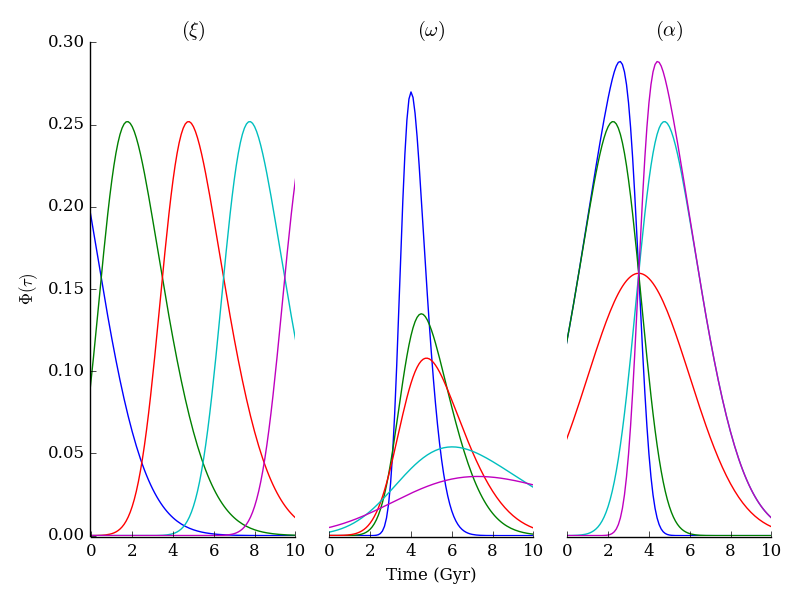
\includegraphics[width=6.5in]{figure_dtd_families}
   \caption{\footnotesize Families of delay-time distributions models shown for various values of location ($\xi$) fixing other parameters (left plot of figure), width ($\omega$, middle plot), and shape ($\alpha$, right plot), for illustration purposes.}
   \label{fig:dtd_families}
\end{figure}

{\bf [ I am HERE]}

\subsection{The Optimized Solution\label{sec:optimized_soln}}
We apply a maximum likelihood estimation method to determine the best-fit unimodal delay time model to Equation~\ref{eqn:std} using a method described in \cite{Hogg:2010fj} and the {\tt emcee.py} documentation~\citep{Foreman-Mackey:2013pd}. We assume, for simplicity, that the errors of all survey data are gaussian in nature, but may be underestimated by some factor ($f$), which may be correctly justified given we are only using the statistical error produced for each value. 

\begin{figure}[t] %  figure placement: here, top, bottom, or page
   \centering
   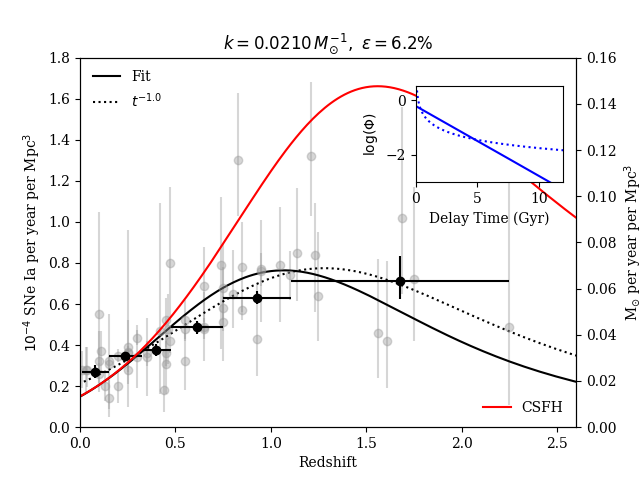
\includegraphics[width=6.5in]{figure_sfd_optimized} 
   \caption{\footnotesize In addition to rate values shown in previous figures, the $R_{\rm Ia}(z)$ result of from optimal parameter fitting is show (black line). The CSFH is shown on in red, and along the secondary abscissa. }
   \label{fig:sfd_optimized_curvefit}
\end{figure}
	
As follows, we adopt the likelihood function to be:
\begin{equation}
\ln p(y|x, \sigma, \varepsilon, \xi, \omega, \alpha, f) = -\frac{1}{2} \sum_i \biggl\{ \frac{[R_{{\rm Ia},i} - {\rm model}(t_i; \varepsilon, \xi, \omega, \alpha)]^2}{s_i^2}+\ln (2\pi s_i^2)\biggr\},
	\label{eqn:lf}
\end{equation}
where,
\begin{equation}
s_i^2 = \sigma_i^2+f^2\, {\rm model}(t_i; \varepsilon, \xi, \omega, \alpha)^2.
\end{equation}
We then find the optimal parameters which maximize this likelihood.

As for priors, we apply rather loose, arbitrary bounds on the optimization, in that we require the successful fraction of progenitors to be between zero and 1, that the width parameters can only be positive, and the that underestimation fraction can only be between zero and 1. Otherwise, the bounds are as follows for parameters $\varepsilon$, $\xi$, $\omega$, $\alpha$, and $\ln f$, respectively: [(0.,1.0),(-2000.,2000.),(0.001,100.),(-500.0,500.0),(-4.,0.)]. The results of that fit are shown in Figure~\ref{fig:sfd_optimized_curvefit}, and in Table~\ref{tab:results}. 


\begin{table}
    \centering
    \caption{Results for unimodal model}
    \label{tab:results}
    \begin{tabular}{cccccc}
        \hline
                Model test & $\varepsilon$ & $\xi$ & $\omega$ & $\alpha$ & $\ln f$ \\ 
                \hline
		CSFH Max.~Likelihood &$0.062$&$-1669.7$& $69.1$& $88.7$& $-2.99$\\
                CSFH MCMC & $0.058^{+0.003}_{-0.007}$ & $-1090^{+1050}_{-650}$ &$54^{+15}_{-40}$& $202^{+203}_{-198}$&  $-2.5^{+1.5}_{-0.9}$\\
                \hline
    \end{tabular}
\end{table}

While the optimization results in values, and a rather interesting delay-time distribution, it is not directly possible to estimate the errors in the parameters via this maximum likelihood optimization method. A Markov chain Monte Carlo (MCMC) is better suited for that.

\subsection{The MCMC solution\label{sec:mcmc_sfd}}
Exploring the parameter space in an MCMC allows both confirmation of the optimized solution and an exploration of the range of validity. We use the affine Invariant MCMC ensemble sampler from {\tt emcee.py}~\citep{Foreman-Mackey:2013pd}, and use the same likelihood function as shown in Equation~\ref{eqn:lf}, and set our uniform priors as described by the bounds, as shown in the previous section. We then set 1,000 walkers to explore 10,000 steps, for a total of 10 million iterations, the first 100,000 of which we discard as `burn-in'. The results of which are shown in Figure~\ref{fig:mcmc_sfd} and Table~\ref{tab:results}.

\begin{figure}[t] %  figure placement: here, top, bottom, or page
   \centering
   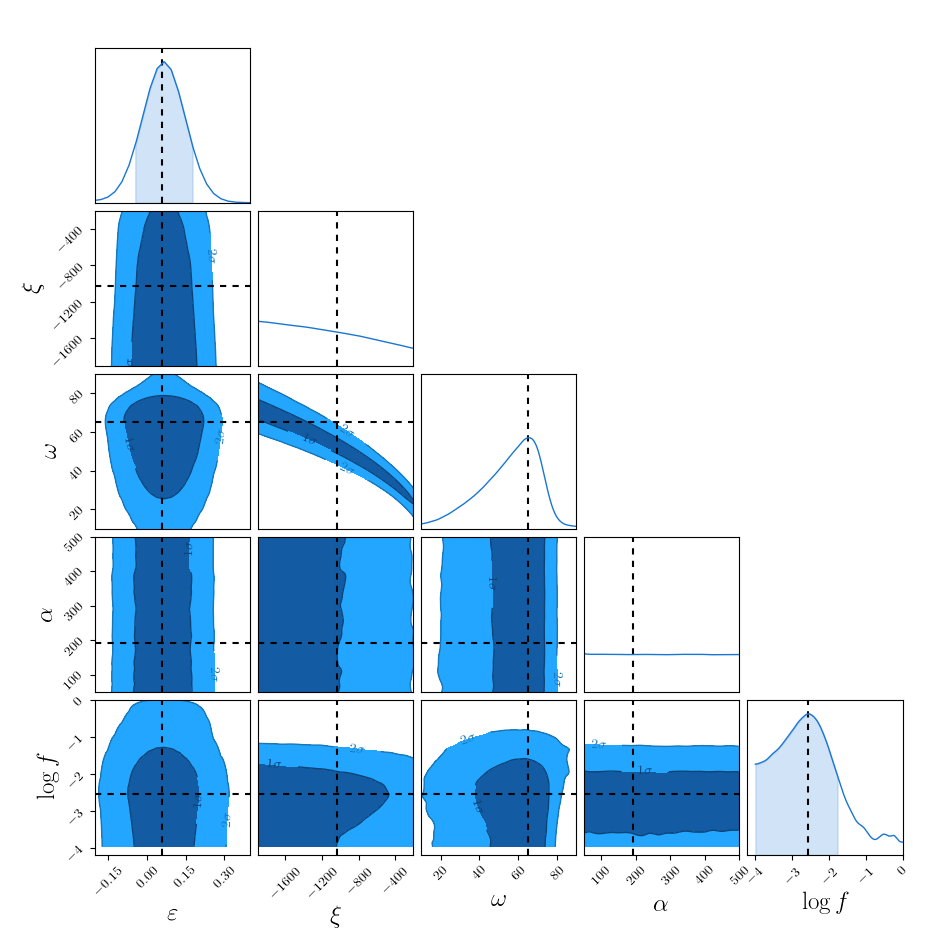
\includegraphics[width=6.5in]{figure_sfd_corners} 
   \caption{\footnotesize MCMC results on unimodal delay-time distribution model, fit to volumetric rate data and CSFH. Plot generated using {\tt ChainConsumer.py} \citep{Hinton:2016qy}.}
   \label{fig:mcmc_sfd}
\end{figure}
\clearpage

\begin{figure}[t] %  figure placement: here, top, bottom, or page
   \centering
   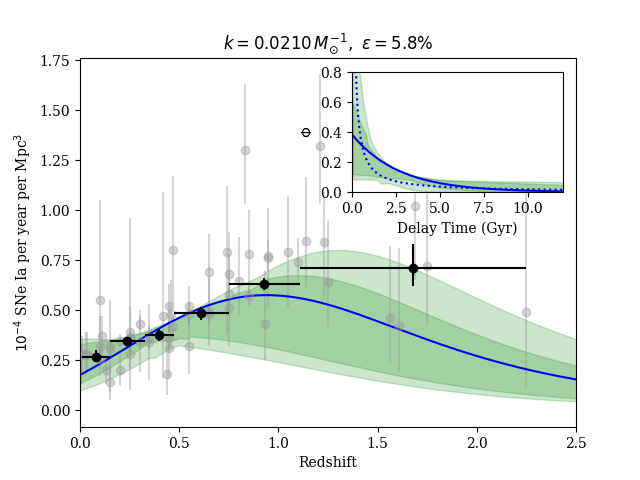
\includegraphics[width=6.5in]{figure_fit_demo_werr} 
   \caption{\footnotesize Similar to Figure~\ref{fig:sfd_optimized_curvefit}, the $R_{\rm Ia}(z)$ result of from MCMC fitting is shown (blue line), with the 68\% confidence interval, in green. }
   \label{fig:figure_fit_demo_werr}
\end{figure}

As is shown, there is a clear convergence in $\ln f$, the factor by which reported errors in rate measures are underestimated. It seems that nearly all values are underestimated by less than 37\%, with most only about 8\% underestimated. While there is a large dispersion in rate values, and seemingly inconsistent rates in some of the same redshift ranges, their values are reasonably consistent with statistical errors, which are not grossly underestimated. Also fairly well constrained is the fraction $\varepsilon$, where only $5.8^{+0.3}_{-0.7}\%$ of WD stars contribute as SN~Ia progenitors. That number increases to  $0.14^{+0.13}_{-0.14}$ when the D18 CSFH is used. However, the parameters we wished to know the most about,  $\xi$, $\omega$, and $\alpha$, appear very much less constrained by the MCMC. There is a clear peak around $\omega\approx60$, but that value is also highly degenerate with the value of $\xi$.  There does not appear to be any convergence or preference in the value of $\alpha$.


While this does not seem to show a clear preference for any specific value set for the model, it does indicate a specific family of solutions that are related. As shown in Figure~\ref{fig:figure_fit_demo_werr}, the 68\% confidence interval about the best fit parameters, all indicate a rather flat DTD. The $t^{-1}$ model is, however, within the 2-$\sigma$ region. 

[NOTE: I should at least talk about Parallel-Tempering Ensemble MCMC, and ...]

\section{Delay Time Distributions from Star Formation Histories}
This is an evaluation of the maximum likelihood delay time distribution following the prescription of \cite{Maoz:2012a} but performed on the GOODS/CANDELS galaxies. For a given galaxy, the rate history of SNe~Ia per year ($r_i$) would be:
\begin{equation}
r_i (t) = h^2\,k\,\varepsilon\, \int_0^t \Psi_i(t')\,\Phi(\tau-t')\,dt',
\label{eqn:rate_history}
\end{equation}
\noindent where $\Psi_i$ is the star formation history of the galaxy (mapped in look-forward time), and $\Phi$ is the global delay time distribution model, also in look-forward time. Figure~\ref{fig:figure_sfh_fit_demo} shows an example ``SN~Ia rate history'' one would derive from Equation~\ref{eqn:rate_history} using the best-fit model from the MCMC on CSFHs, done in the previous sections.

The product of the rate at the observed epoch ($r_{i,0}$) and the observed control time ($t'_{c, i}$) of the galaxy-- which contains all the information on the temporal sampling and depth of the survey--  give ($m_i$) the expected number of observed SN~Ia events over the duration of the survey, or
\begin{equation}
m_i = r_i \, t'_{c, i}.
\end{equation}
\noindent The probability distribution of those observed events is likely Poisson, where of catching $n_i$ SNe~Ia from that galaxy when $m_i$ are expected is
\begin{equation}
P(n_i | m_i) = \frac{m_i^{n_i}e^{-m_i}}{n_i!}.
\end{equation}
\noindent The product of probabilities for all galaxies in the survey would then serve as the likelihood of a given delay-time distribution model. The log-likelihood, convenient for MCMCs, is then expressed by:
\begin{equation}
L = \prod _i^N P(n_i|M_i) \Rightarrow \ln L = -\sum^N m_i+\sum^N\ln\biggl(\frac{m_i^{n_i}}{n_i!}\biggr)
\end{equation}
\noindent in which the last term is zero for the galaxies which did not host SNe~Ia during the survey.


\begin{figure}[t] %  figure placement: here, top, bottom, or page
   \centering
   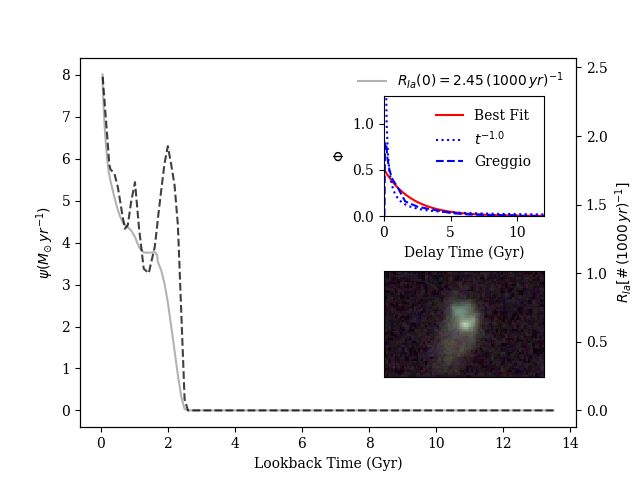
\includegraphics[width=6.5in]{figure_sfh_demo_v2} 
   \caption{\footnotesize Similar to Figure~\ref{fig:sfd_optimized_curvefit}, the $R_{\rm Ia}(z)$ result of from MCMC fitting is shown (blue line), with the 68\% confidence interval, in green. }
   \label{fig:figure_sfh_fit_demo1}
\end{figure}
\begin{figure}[t] %  figure placement: here, top, bottom, or page
   \centering
   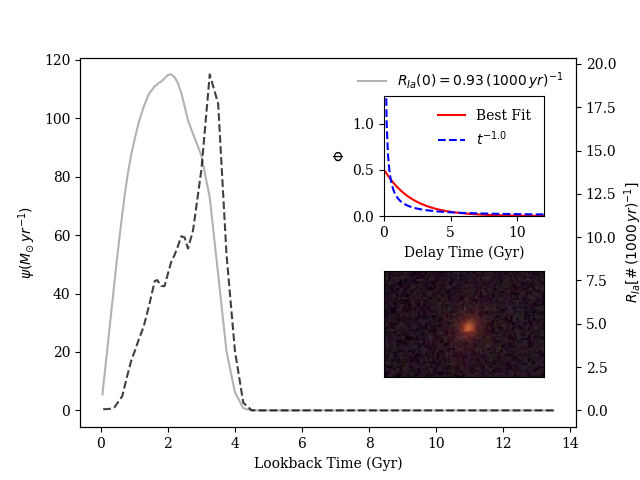
\includegraphics[width=6.5in]{figure_sfh_demo_v1} 
   \caption{\footnotesize Similar to Figure~\ref{fig:sfd_optimized_curvefit}, the $R_{\rm Ia}(z)$ result of from MCMC fitting is shown (blue line), with the 68\% confidence interval, in green. }
   \label{fig:figure_sfh_fit_demo2}
\end{figure}

Examples of this are shown in Figures~\ref{fig:figure_sfh_fit_demo1} and \ref{fig:figure_sfh_fit_demo2}. 
There are 34 events we classified as SNe~Ia in the GOODS/CANDELS South field, and 39 in the North field, all but 6 of which were matched to a host galaxy in the SFH catalog. Two were rejected as the host redshifts were inconsistent with the catalog redshifts, and another 4 were rejected as they were not in the catalog, largely as they were either too faint or near the field edge to be listed in their composite photometry catalogs. 


The model parameters, $\xi$, $\omega$, and $\alpha$ is then explorable via {\tt emcee.py}. We keep the same uniform priors as bounds, as described in Sections~\ref{sec:optimized_soln} and \ref{sec:mcmc_sfd}.


\begin{figure}[t] %  figure placement: here, top, bottom, or page
   \centering
   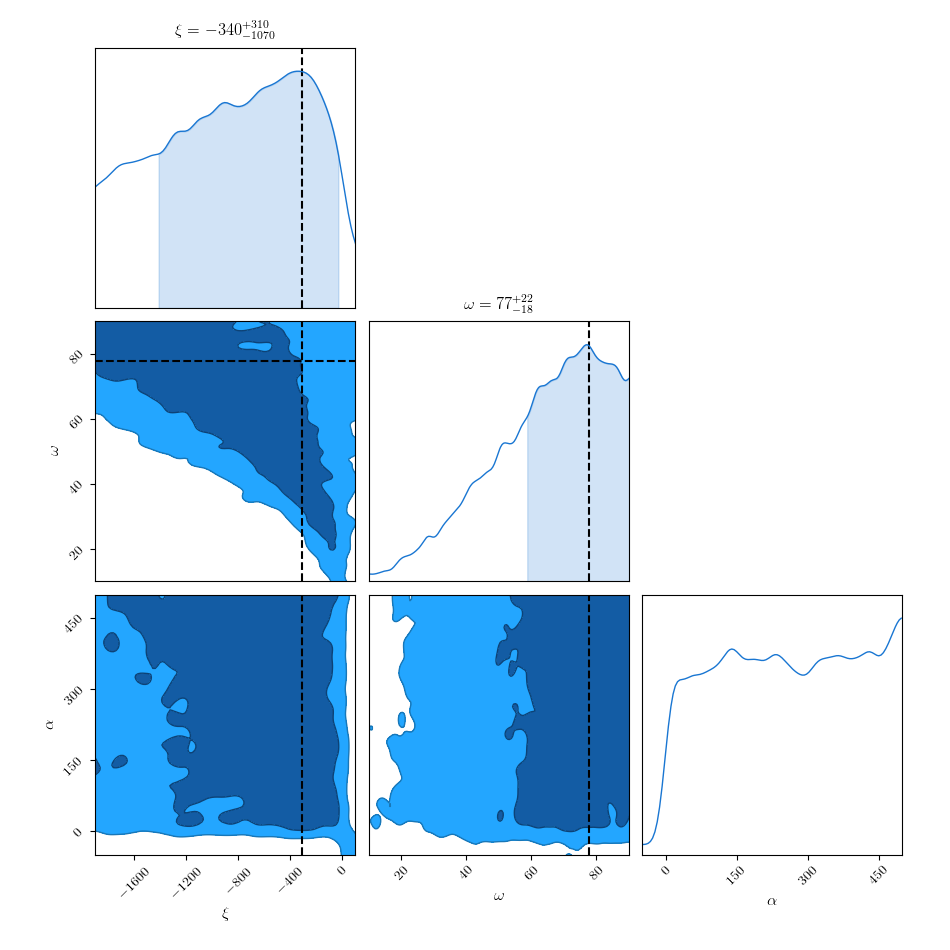
\includegraphics[width=6.5in]{figure_sfh_corners} 
   \caption{\footnotesize MCMC results on unimodal delay-time distribution model, fit to SFHs for 147 galaxies in CANDELS, 49 of which are SN~Ia hosts.}
   \label{fig:mcmc_sfd}
\end{figure}

\section{discussion}

\bibliography{strolger}{}

\begin{table}
    \centering
    \caption{Parameter Covariance MCMC SFD}
    \label{tab:parameter_covariance}
    \begin{tabular}{c|ccccc}
         & $f$ & $\xi$ & $\omega$ & $\alpha$ & $\log \phi$\\ 
        \hline
              $f$ &  0.41 & -125.69 &  6.61 & 33.98 & -0.41 \\ 
            $\xi$ & -125.69 & 412816.10 & -14898.10 & -52398.20 & 518.74 \\ 
         $\omega$ &  6.61 & -14898.10 & 660.60 & 2209.32 & -22.89 \\ 
         $\alpha$ & 33.98 & -52398.20 & 2209.32 & 27290.24 & -131.67 \\ 
        $\log \phi$ & -0.41 & 518.74 & -22.89 & -131.67 &  2.35 \\ 
        \hline
    \end{tabular}
\end{table}


\end{document}